\setRL
%\pagenumbering{arabic} 



\subsection{
شکل کره‌ی دارای نقطه‌ی نقص
}
حدود ۴۰۰ سال پیش اویلر به مسئله‌ی مثلث بندی کردن سطوح فکر کرده بود و روابطی برای برای ارتباط تعداد رئوس (یا نقاط)، اضلاع، و وجوه مش‌های مثلث بندی روی کره ارائه داده‌است.  بنا به نظریه‌ی اویلر، اگر فرض کنیم که درجه‌ی رئوس (تعداد وجوهی که به رئوس ختم می‌شوند) رئوس مش مثلثی یک سطح بسته فقط ۵، ۶، و ۷ باشد، کمترین اختلاف تعداد رئوس نقص (۵ و ۷) روی سطح با جینوس سطح رابطه دارد:
\begin{equation}
N_D=N_5-N_7=12(1-g)
\label{eq:genus}
\end{equation}
که در اینجا
$N_D$
اختلاف تعداد نقاط نقص و 
$g$
جینوس
\LTRfootnote{genus}
 سطح است. جینوس سطح بسته تعداد دسته‌هایی است که در آن شکل وجود دارد. مثلا کره سطح بسته‌ایست که دسته ندارد و چنبره سطحی است که یک دسته دارد. اگر فرض کنیم که مش مثلثی‌ فقط از رئوس با درجه‌ی ۵ و ۶ ساخته شده باشد، در این صورت کمترین نقاط نقص با درجه‌ی ۵ که می‌توان بر روی سطح داشت، ۱۲ خواهد بود (شکل
 \ref{fig:genus}
 ).
\begin{figure}[h]
\begin{center}
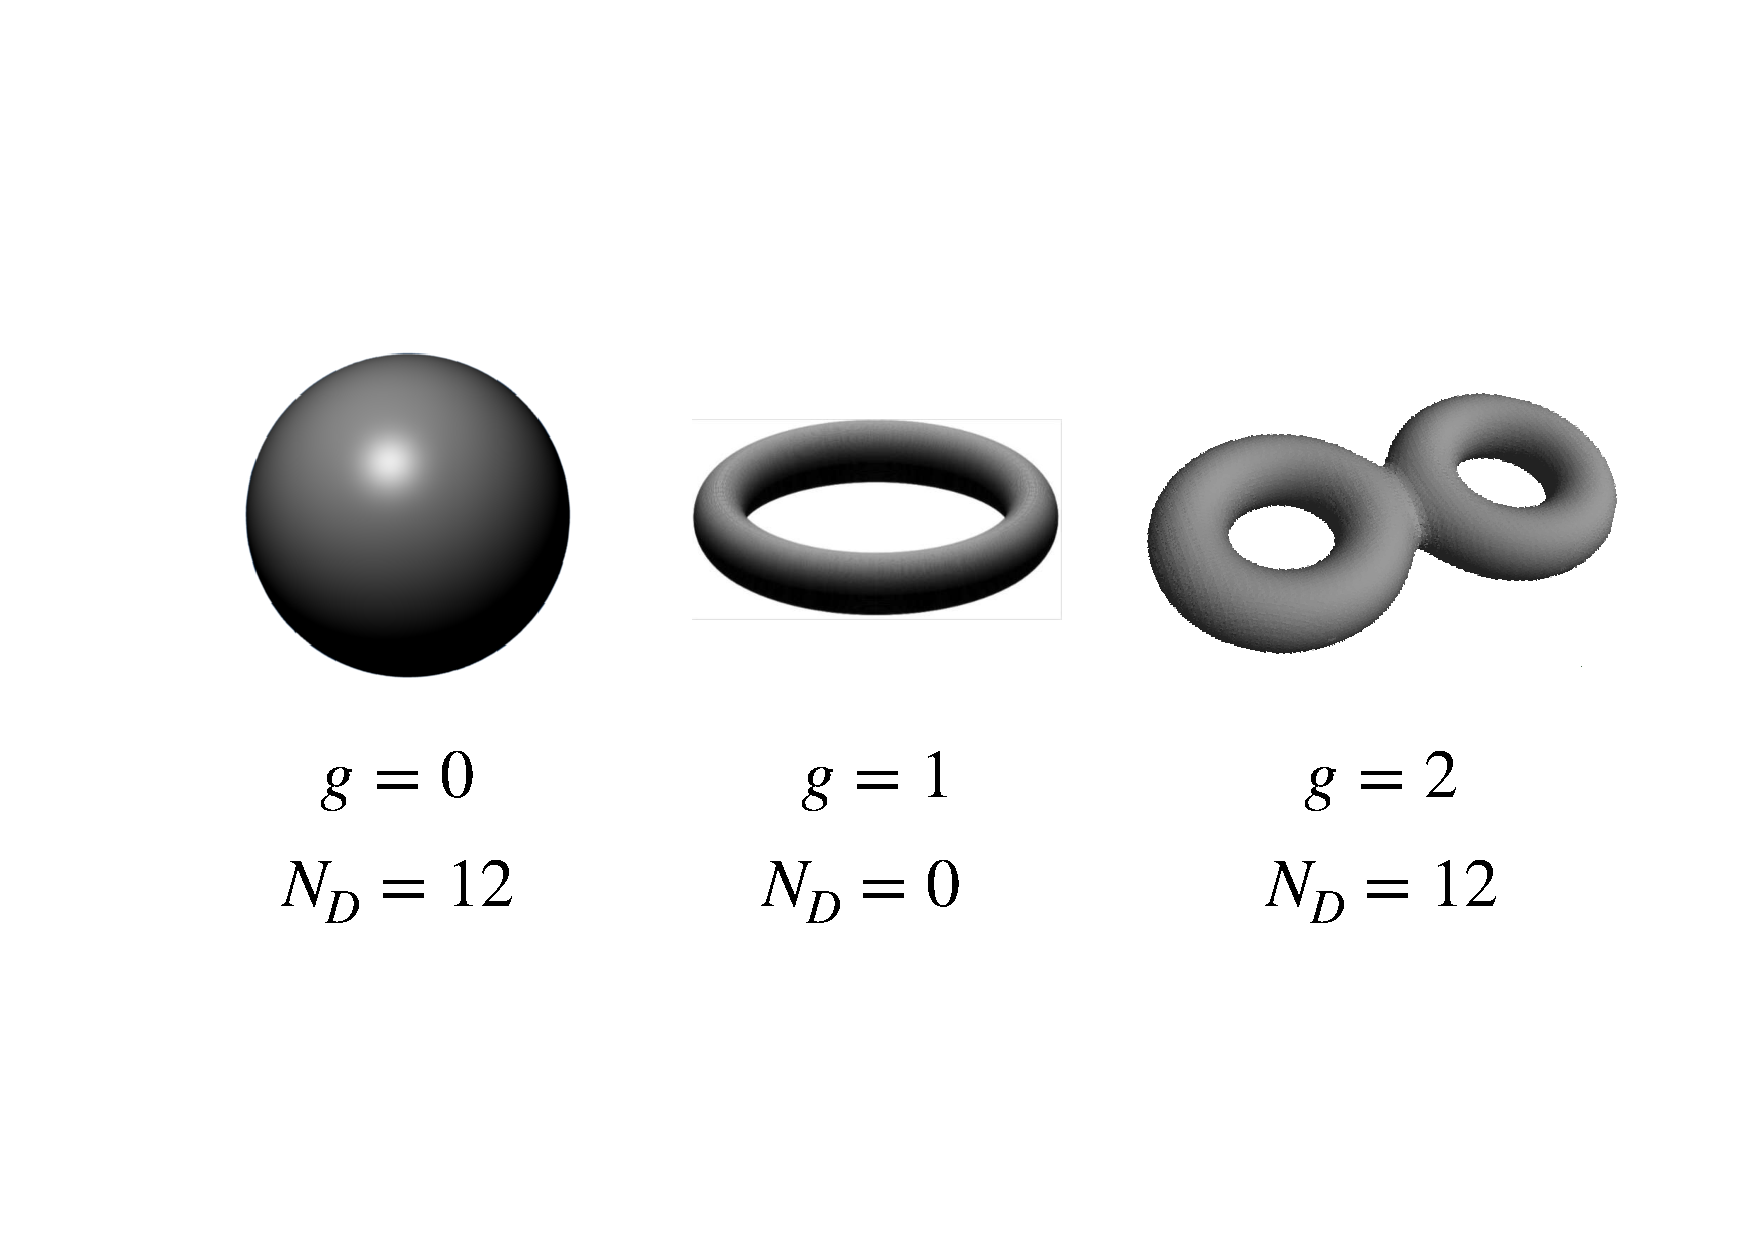
\includegraphics[width=6in]{\MemModel/Pics/genus.pages.pdf}
\caption{
۳ مثال از سطوح بسته به همراه جینوس و کمترین تعداد نقاط نقص لازم  برای ساخت آن با مش مثلثی.
}
\label{fig:genus}
\end{center}
\end{figure}


معادلات
\ref{eq:stretchdiscenergy}
و
\ref{eq:bendingdiscenergy}
تغییر انرژی کششی و خمشی یک مش منظم پس از اضافه شدن نقص به مرکز شبکه را توصیف می‌کنند. رقابت میان این دو جمله تعیین می‌کند که یک مش مثلثی کروی به لحاظ انرژی چه شکلی را به خود می‌گیرد. با مقایسه‌ی این دو جمله می‌توان عدد بی بعد  فاپل فون کارمان
\LTRfootnote{Foppl–von Kármán number}
را ساخت
\cite{nelsonPRE2003}
:
\begin{equation}
\gamma = \frac{Y_{2D}R^2}{\kappa}
\label{eq:gamma}
\end{equation}
اگر تمام اضلاع یک مش مثلثی کروی از یک جنس باشند (مدول یانگ و طول اولیه یکسان) در این صورت، عدد فاپل فون کارمان شکل نهایی مش را تایین می‌کند. برای مقادیر زیاد، هزینه‌ی کشش فنر‌ها نسبت به خم شدن بیشتر است و حالت کمینه‌ی انرژی آزاد مجموعه زمانی‌ است که طول تمام اضلاع به طول اولیه‌ خود (انرژی کششی کم) بسیار نزدیک است. از آنجایی که سطح دو بعدی است و قید بسته بودن دارد، به ناچار خمش در محل‌های مشخصی ایجاد می‌شود. از آنجایی که تعداد همسایه‌های مثلث‌های نقاط نقص (۵) کمتر از همسایه‌های مثلث‌های جاهای دیگر (۶) است، هزینه‌ی خم شدن در این نقاط کمتر از جاهای دیگر است و کره شکل بیست‌وجهی
\LTRfootnote{icosehedron}
به خود می‌گیرد.
به همین ترتیب در حد اعداد فاپل فون کارمان کوچک هزینه‌ی کشش در سیستم کم است و سیستم شکل کروی (کمترین خمش) به خود می‌گیرد. در شکل
\ref{fig:gamma}
هندسه‌ی مش مثلثی بسته با ۱۲ نقطه‌ی نقص با گاماهای مختلف نشان داده شده است. در گاماها‌ی کوچک (۴۵) هندسه کروی‌است. این هندسه تا مقدار ۱۵۴ (که مقدار حدی تغییر شکل مش است
\cite{nelsonPRE2003}
) حفظ می‌شود. برای مقادیر گامای بیشتر از ۱۵۴ شکل کره دیگر شکل کمینه‌ی سیستم نخواهد بود و هندسه به طور پیوسته با افزایش گاما به شکل ۲۰ وجهی تغییر می‌کند.
\begin{figure}[h]
\begin{center}
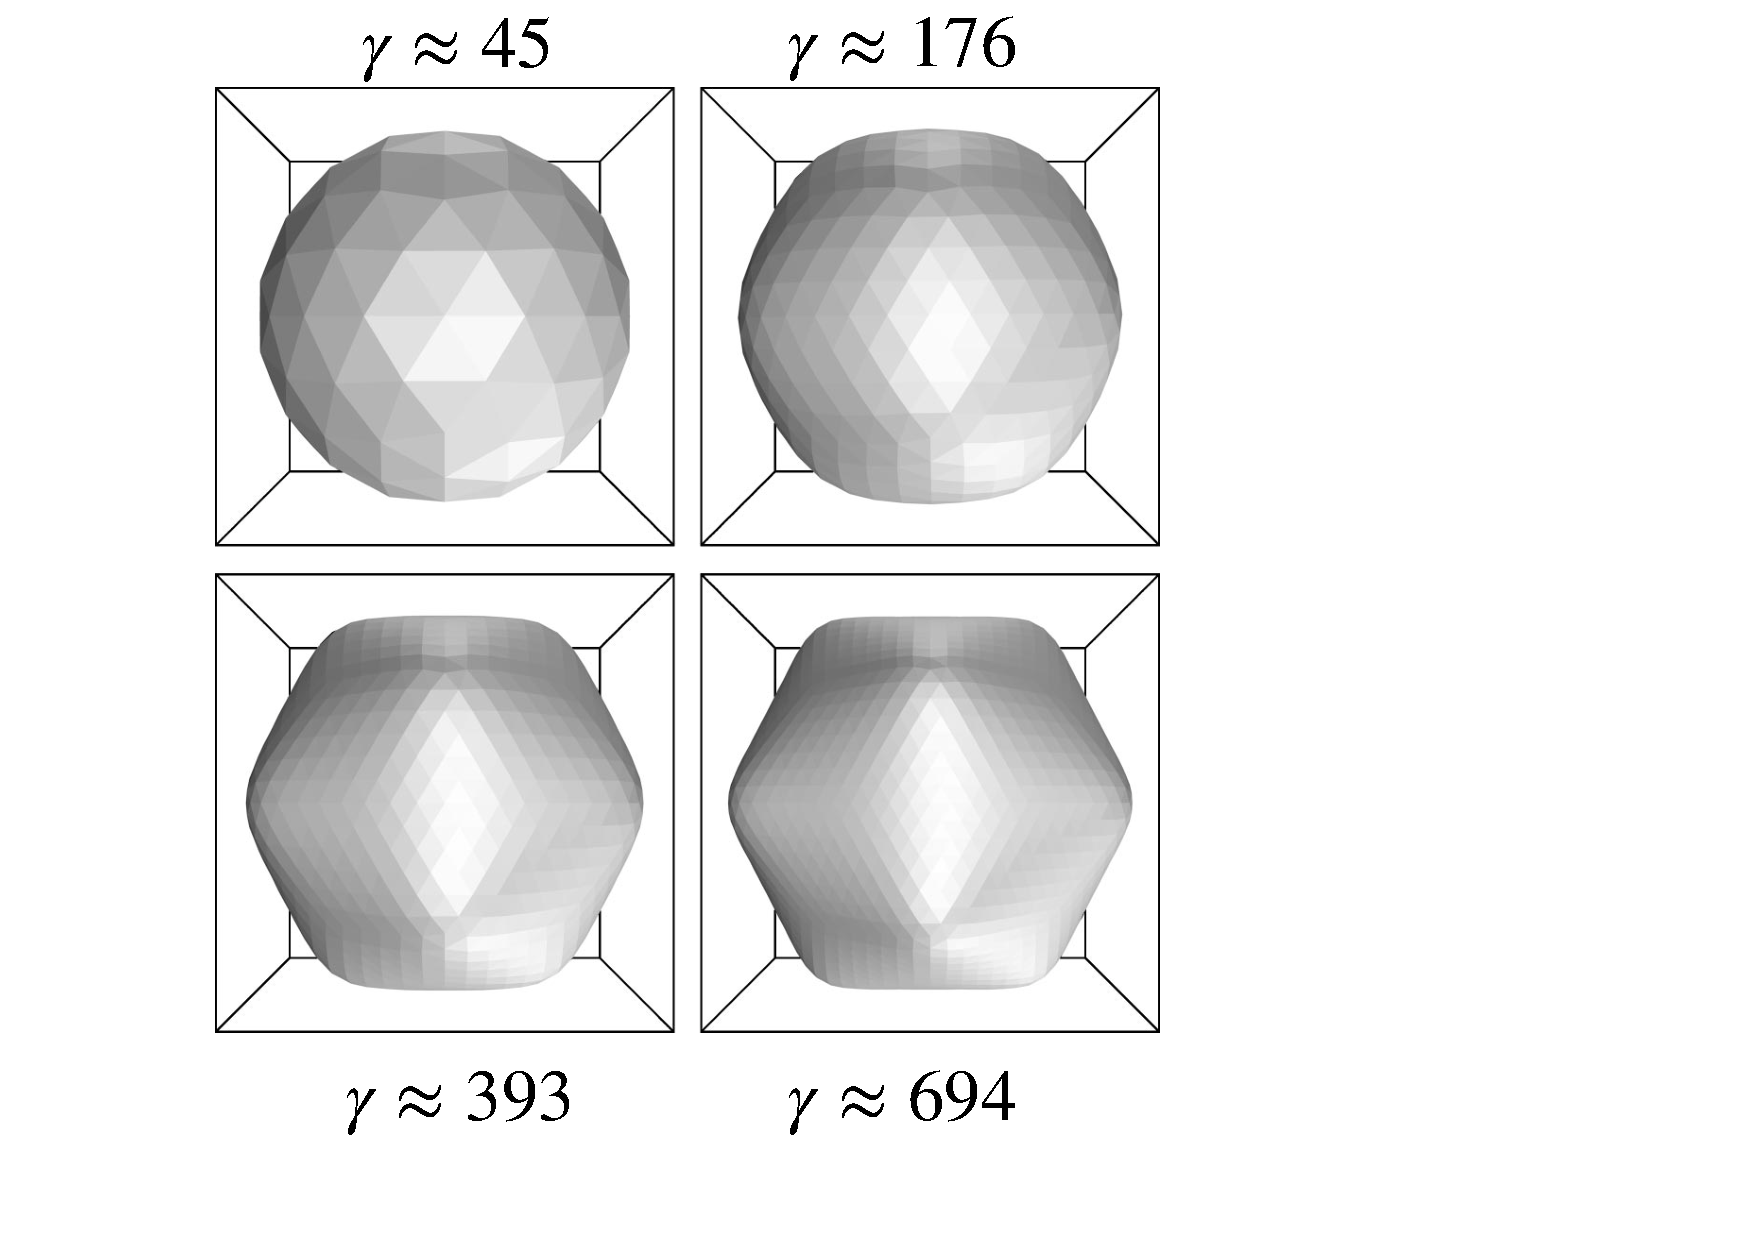
\includegraphics[width=4in]{\MemModel/Pics/gamma.pages.pdf}
\caption{
مثال‌هایی از شکل کمینه انرژی مش مثلثی کروی درجه‌ی ۶ با ۱۲ نقطه‌ی نقص. گاما عدد فاپل فون کارمان است. برای مقادیر کم گاما شکل بهینه، کره است و برای مقادیر بالاتر مقدار حدی ۱۵۴، شکل بهینه بیست وجهی است.
}
\label{fig:gamma}
\end{center}
\end{figure}
لازم است تاکید شود که گاما به غیر از مدول‌های الاستیک به اندازه‌ی سطح نیز وا بسته است. در نتیجه در صورتی که مش مثلثی با مدول الاستیک مشخصی ساخته شود، با تنظیم اندازه‌ی مش (یا طول اضلاع) شکل بهینه‌ی سیستم را می‌توان تغییر داد.







